%{\color{red}
%• Os protótipos de baixo nível (em papel) usado para definir o projeto da aplicação, caso 
%tenham sido usados. }

%{\color{red}
%• Um protótipo em wireframe do sistema, com as justificativas (baseadas nos princípios 
%de usabilidade, conceitos de design e nas metas estabelecidas no item 1) para a 
%escolha e alocação de cada elemento de interface. }

%\subsection{Protótipo de baixo nível}  {\color{red} OK -- não foi utilizado }
%\subsection{Protótipo de alto nível}

Para a criação dos protótipos foi utilizado o \emph{software} de 
prototipação Fluid UI criado por Kearney e Hannigan em 2010,
disponível \emph{online}\footnote{Disponível em:
<https://www.fluidui.com/>. Acesso em: 28 abr. 2013.}.
A figura \ref{fig:TelaHistorico} mostra os \emph{mockups} para a tela de
consultas já realizadas, do lado esquerdo, e a tela de uma
consulta em andamento, do lado direito.  A figura
 \ref{fig:TelaHarryPotter} mostra os \emph{mockups} para as telas de resultado.
 Ao lado esquerdo a tela de uma busca bem sucedida, com a foto
 da capa encontrada \emph{online}, o título e a avaliação da
 comunidade, com os preços logo em seguida.  Ao lado direito
 está a tela de busca mal sucedida, onde uma mensagem de erro é mostrada
 solicitando o usuário a tirar uma nova foto.  No caso de uma busca mal
 sucedida, o usuário pode ter tirado uma foto de forma inadequada,
 como mostrada na figura, onde a foto está borrada pelo movimento
 praticado pelo usuário durante a captação da imagem.

Os protótipos desenvolvidos utilizam listas, botões, diálogos e imagens.
Um botão consiste de um texto que comunica claramente a ação que será
tomada quando o usuário o toca.   Neste \emph{design} foi utilizado apenas
um botão, com bordas para facilitar a identificação do artefato como
botão.  
Um diálogo é um pedido ao usuário para tomar uma decisão de controle ou
oferecer informações adicionais necessárias para que a aplicação continue
sua tarefa.  Tais pedidos podem ser desde decisões de OK/Cancelar para
leiautes mais complexos que pedem ao usuário ajustes de configurações
adicionais. Por fim,
uma lista apresenta múltiplos itens em várias linhas dispostas em um
leiaute vertical.  Listas são utilizadas para seleção de dados ou para
a navegação de dados sendo visualizados.

%{\color{red} justificar cada elemento da interface }
\begin{figure}[ht]
        \begin{minipage}{.5\textwidth}
            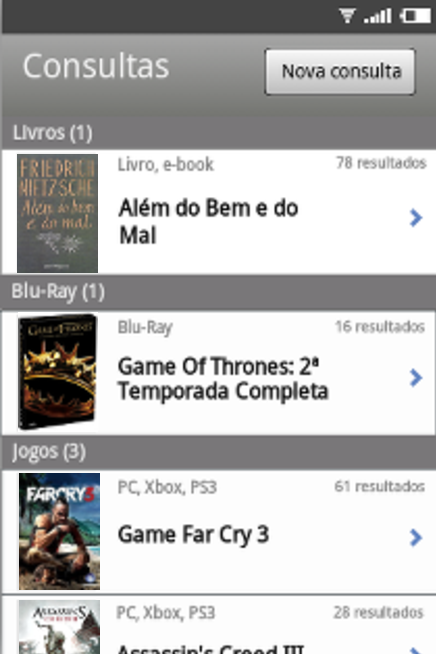
\includegraphics[scale=1]{tela/TelaHistorico}
        \end{minipage}
        \begin{minipage}{.5\textwidth}
            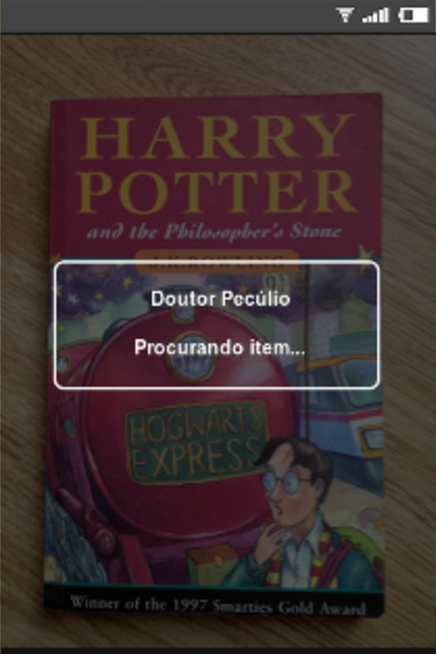
\includegraphics[scale=1]{tela/TelaBuscando}
        \end{minipage}
        \caption{ \label{fig:TelaHistorico} \textit{Mockups} para telas de 
            histórico de consultas e uma consulta em andamento. }

        \begin{minipage}{.5\textwidth}
            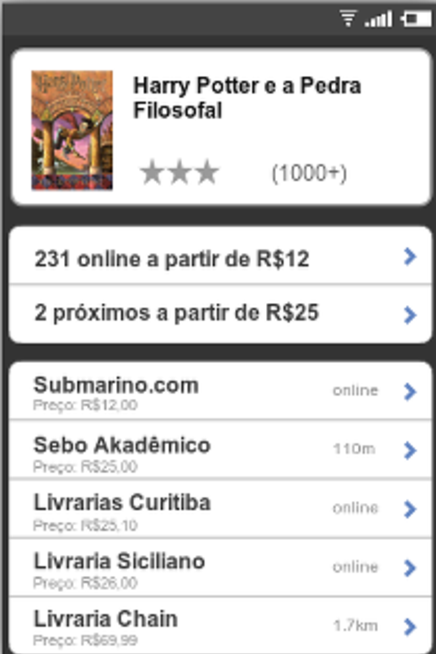
\includegraphics[scale=1]{tela/Tela}
        \end{minipage}
        \begin{minipage}{.5\textwidth}
            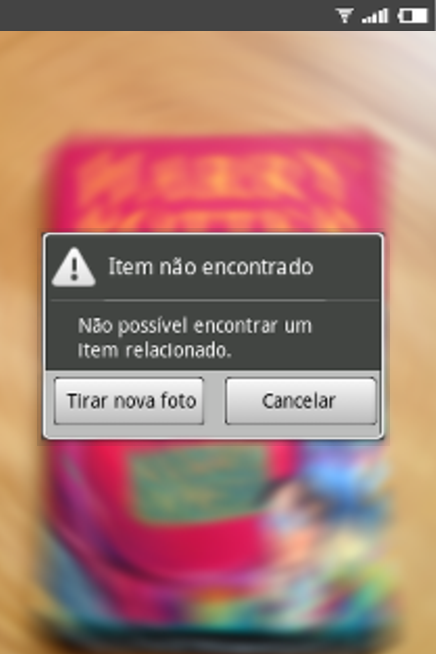
\includegraphics[scale=1]{tela/TelaErro}
        \end{minipage}
        \caption{ \label{fig:TelaHarryPotter} \textit{Mockups} para telas de 
            resultados bem e mal sucedidos. }
\end{figure}
